\xchapter{Methodology}{}

In this chapter, we present formulations to the many variants of the source code attribution problem in section \ref{sec:formulations}, we describe how the Codeforces dataset was assembled in section \ref{sec:dataset} and present a top-down approach to how the end-to-end model was developed in section \ref{sec:framework}.

\section{Problem Formulations}\label{sec:formulations}
\section{Datasets}\label{sec:dataset}

The first step to develop an effective deep learning model is to gather enough training data. In this work, we decided to work with C++ source codes written in a laboratory environment -- we assume the whole code is written by the author under no external style enforcement such as a style guide.

\subsection{Google Code Jam}

Although there are many public C++ laboratory datasets, the Google Code Jam\footnote{\url{https://codingcompetitions.withgoogle.com/codejam}} dataset \cite{caliskan_2015} is probably the biggest of them all. Samples from this dataset are collected from previous editions of Google Code Jam, an annual programming competition held by Google. In this competition, participants are given algorithmic tasks to be solved in a limited amount of time. As such, it's very likely that code written by a participant manifests his own coding style.

Google Code Jam holds nearly 10 rounds every year. Most of these rounds are eliminatory. Thus, the availability of samples from less experienced participants is expected to be low. If we want to build a balanced training set not biased by the way experienced participants code, we are limited by the small amount of code less experienced participants wrote.

Although this dataset was not extensively used throughout the development phase, it was a reference for the Codeforces dataset introduced in section \ref{sec:codeforces}.

\subsection{Codeforces}\label{sec:codeforces}

Codeforces\footnote{\url{http://codeforces.com}} is a website specialized in holding online programming contests. Contest format is similar to Google Code Jam's, but they are not eliminatory. Thus, we are able to find a lot of samples from both non-experienced and experienced users.

We wrote a Python script that receives target constraints for the dataset and scrapes Codeforces for samples. Using this script, we assembled a balanced dataset with more than 30,000 samples from nearly 2,000 authors, meaning that we have around 15 samples per author. This dataset was packaged and made public\footnote{link-pro-dataset}.
% TODO: more details on filters
% TODO: add link to dataset

\section{Source Code Embedding Model}\label{sec:framework}

In this section, we propose a deep learning model that embeds source codes, from their string representations, into a denser latent space. In section \ref{sec:descriptor}, we describe what is a style descriptor. In section \ref{sec:models}, we describe network architectures used in our work. In section \ref{sec:optimization}, we describe how the network was trained to generate meaningful style descriptors.

\begin{figure}[ht]
	\centering
	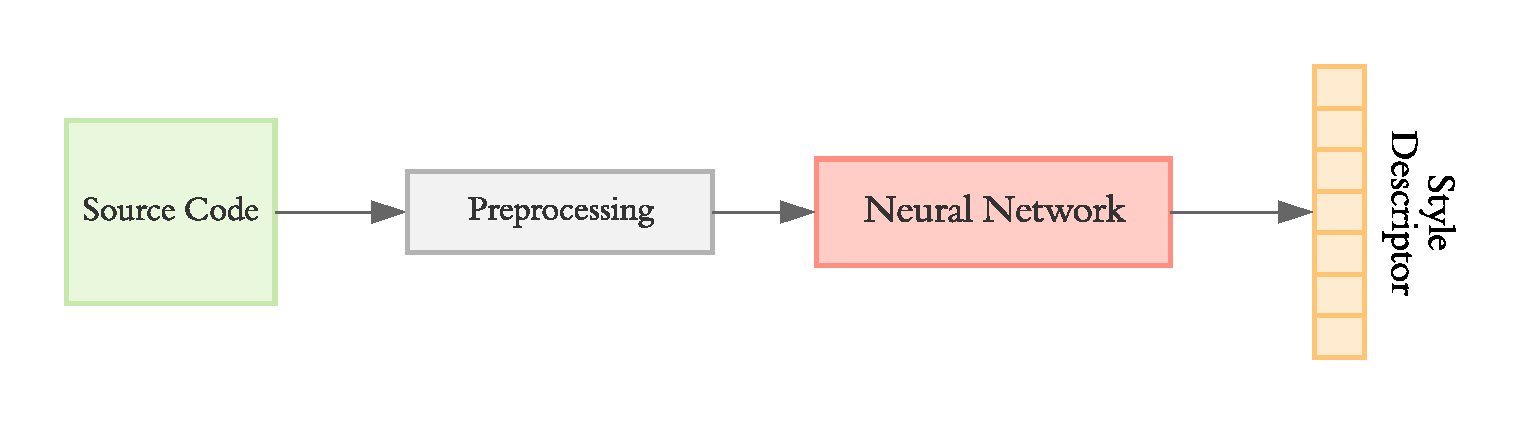
\includegraphics[width=\linewidth]{imgs/lstm.pdf}
	\caption{Overview of style descriptor generation pipeline.}
	\label{fig:overall}
\end{figure}

\subsection{Coding Style Descriptor}\label{sec:descriptor}

The performance of machine learning methods is heavily affected by the choice of data representation. Thus, much of the effort of the machine learning community has been put into developing algorithms that transform otherwise unmanageable data into representations that can be effectively used by learning methods \cite{representation_learning}.

A Coding Style Descriptor (hereon referred simply as \textit{style descriptor}) is an $n$-dimensional representation of a source code in a latent space. A latent space is a space where representations of similar objects lie close to each other. Therefore, the latent space of style descriptors captures stylistic similarities of source codes. Ideally, style descriptors should encode everything a machine learning model needs to solve the problems posed in section \ref{sec:formulations}. Thus, we can build simpler classifiers for these problems if we are able to build good latent representations for source codes.

% TODO: add image explaining this concept
% TODO: add references to embedding being succesfully applied in conjunction with deep learning

Deep feed-forward networks are a natural approach to representation learning. In the remainder of this chapter, we will mainly study deep learning techniques to generate style descriptors from source codes.

\subsection{Models}\label{sec:models}
\subsubsection{Char-Level CNNs}
\paragraph*{Network Architecture}
\subsubsection{Hierarchical LSTMs}
\paragraph*{Network Architecture}

\subsection{Optimization}\label{sec:optimization}

